\chapter[Proposta]{Proposta}
\label{cap:proposta}

Esse capítulo aborda a proposta principal deste trabalho. Inicialmente, será apresentada uma breve 
Contextualização (\ref{section:proposta_context}) seguida da descrição do escopo a ser desenvolvido 
pelos autores (\ref{section:escopo}), utilizando da reengenharia e das técnicas do TDD e do DDD, descritas 
no Referencial Teórico (\ref{cap:referencial}). Será utilizada a "Metodologia Orientada a Provas de 
Conceito" conforme item \ref{section:metod_poc}, demonstrado nos tópicos \ref{section:poc_1}, 
\ref{section:poc_2}, \ref{section:poc_3} e \ref{section:poc_4}, onde a prova de 
conceito é descrita com sua respectiva definição do desafio e dos seus requisitos. Além disso, no que diz respeito à 
POC 1 (\ref{section:poc_1}), são realizadas a Apresentação da Solução (\ref{subsection:apresentacao_solucao}) 
e a Análise dos Resultados (\ref{subsection:analise_resultados}). Por último, encontram-se as Considerações 
Finais do Capítulo (\ref{section:consideracoes_finais_proposta}).

\section{Contextualização}
\label{section:proposta_context}

Conforme discutido anteriormente neste trabalho, o aplicativo \citeauthoronline{MiaAjuda} (\citeyear{MiaAjuda}) foi desenvolvido em 2020, 
durante o início da pandemia de Covid-19, com o objetivo de conectar usuários que necessitam de apoio, 
oferecendo uma plataforma para que pessoas possam solicitar e oferecer ajuda, seja ela de natureza material 
ou emocional. Devido à realidade desafiadora da pandemia, a demanda por soluções de cunho social aumentou 
drasticamente, levando o aplicativo a ter uma urgência no prazo de sua construção. Com isso, o processo de 
desenvolvimento da aplicação não atendeu os critérios definidos como boas práticas pela comunidade de 
\textit{software}, deixando uma margem para possíveis evoluções.

O \textit{Design} de \textit{Software} é um processo fundamental para o desenvolvimento de um sistema, 
por ser o detalhamento de mais baixo nível com um conjunto de princípios, normas e técnicas. Sem 
ele, o \textit{software} fica suscetível a diversos problemas futuros relacionados à manutenção e 
evolução do mesmo \cite{robert2019clean}.

A escolha das técnicas de programação que serão utilizadas no desenvolvimento de um 
\textit{software} é fundamental para garantir a qualidade, manutenibilidade e eficiência 
do código fonte. Existem diversas técnicas de programação dentro da Engenharia de \textit{Software}, 
com várias particularidades. Diante disso, é necessário uma boa escolha das técnicas que serão 
utilizadas no desenvolvimento, a fim de implementar uma solução eficaz, confiável e de desempenho 
adequado.

Ante o exposto, a técnica de programação do TDD, que visa uma melhor testabilidade, e o DDD, que define um 
\textit{design} de \textit{software} que reflete exatamente suas funcionalidades, são abordagens possíveis 
para a reengenharia de um aplicativo, visando a evolução do mesmo.


\section{Escopo}
\label{section:escopo}

Com o objetivo de realizar a reengenharia do aplicativo \citeauthoronline{MiaAjuda} (\citeyear{MiaAjuda}), aplicando os conceitos definidos 
no capítulo de Referencial Teórico \ref{cap:referencial} do trabalho, optou-se pelo desenvolvimento de uma parte 
das funcionalidades presentes na aplicação.

O escopo definido não compreende o aplicativo em sua totalidade por ter o objetivo de avaliar 
a testabilidade facilitada e a adequada modelagem de domínio, não sendo necessária a implementação total do 
aplicativo. No sistema em desenvolvimento neste trabalho, os usuários podem solicitar uma ajuda e também oferecer 
ajuda às solicitações existentes, sendo funcionalidades já implementadas no aplicativo.

Com o desenvolvimento de cada funcionalidade, é relevante avaliar: (i) se o domínio está adequadamente 
modelado; (ii) se é fácil testá-la e se a mesma está com uma boa cobertura de testes, e (iii) se é fácil 
incorporar novas funcionalidades sem comprometer o \textit{design} de \textit{software} estabelecido. A 
partir dos resultados obtidos e avaliados, espera-se responder às Questões de Pesquisa e de Desenvolvimento \ref{section:questoesdepesquisa}  
estabelecidas para este trabalho.

O sistema em desenvolvimento é composto por três módulos: Autenticação de Usuário; Solicitar Ajuda; 
e Oferecer Ajuda. Cada módulo compreende um domínio da aplicação, e deverá ser desenvolvido utilizando 
a abordagem combinada de TDD e DDD.


\section{POC 1}
\label{section:poc_1}

Essa seção aborda a configuração do ambiente de desenvolvimento do sistema, 
além do desenvolvimento de uma rota de verificação.  No primeiro momento, 
é apresentada a Definição do Desafio \ref{section:poc_1_def_desafio} atrelada a essa prova de conceito, 
seguido pelos Requisitos do Desafio \ref{section:poc_1_req_desafio}.

\subsection{Definição do Desafio}
\label{section:poc_1_def_desafio}

Tem como objetivo estabelecer todo o ambiente de desenvolvimento, configurando as 
tecnologias e ferramentas estabelecidas, além de desenvolver, utilizando TDD e 
DDD, uma primeira rota para verificação da saúde do sistema.

\subsection{Requisitos do Desafio}
\label{section:poc_1_req_desafio}

Para que a prova de conceito seja considerada finalizada, é necessário cumprir os seguintes requisitos:

\begin{itemize}
  \item O sistema deve ser acessível através de um \textit{host};
  \item O sistema deve ser capaz de gerar insumos a respeito de sua qualidade, e 
  \item O usuário deve ser capaz de verificar a saúde do sistema.
\end{itemize}

\subsection{Apresentação da Solução}
\label{subsection:apresentacao_solucao}

No primeiro momento dessa solução, tem-se a configuração do ambiente de desenvolvimento, 
sendo necessário iniciar o serviço \textit{server-side} com o \textit{framework} estabelecido para 
implementação. Depois, é necessário inicializar as ferramentas e bibliotecas escolhidas para 
implementação e análise de código. Com o ambiente configurado, o serviço deve ser capaz de atender 
requisições HTTP feitas a ele por \textit{clients}.

No segundo momento, tem-se a implementação de uma rota na qual disponibiliza informações 
sobre a aplicação, se a mesma está disponível e por quanto tempo ela se 
encontra disponível. Para esta parte da solução, é necessário utilizar a linguagem de 
programação e biblioteca de testes estabelecidas para o desenvolvimento, além de utilizar o TDD e o DDD.

\subsubsection{Configuração do Ambiente}

Para a configuração do ambiente de desenvolvimento, primeiro iniciou-se o projeto utilizando o 
\textit{framework} Express \footnote{https://expressjs.com/. Acessado pela última vez em 09/12/2023.} que tem o 
Node \footnote{https://nodejs.org. Acessado pela última vez em 09/12/2023.} como base, como foi estabelecido no capítulo de Suporte 
Tecnológico \ref{cap:suporte}. Depois, configurou-se a ferramenta SonarQube \footnote{https://docs.sonarsource.com/sonarqube/latest. Acessado pela última vez em 09/12/2023.}, 
responsável por analisar a qualidade do código fonte e gerar insumos para a análise quantitativa 
das POCs. Em seguida, foi feita a configuração do Docker \footnote{https://www.docker.com. Acessado pela última vez em 09/12/2023.} juntamente com o banco 
de dados MongoDB \footnote{https://www.mongodb.com. Acessado pela última vez em 09/12/2023.} e o Firebase \footnote{https://firebase.google.com. Acessado pela última vez em 09/12/2023.}, para a conteinerização do serviço 
e armazenamento de dados. Com isso, ao iniciar o serviço, tem-se um \textit{host} disponível para 
requisições HTTP.s

\subsubsection{Rota de Verificação}

Com o objetivo de validar o ambiente criado e criar uma base para a implementação com TDD e DDD, criou-se uma 
rota para verificação do sistema. Utilizando a técnica do TDD, primeiramente houve a implementação dos testes 
unitários para esta funcionalidade. A Figura \ref{fig-poc1-code-test} evidencia um dos testes criados para a funcionalidade.

\begin{figure}[h]
	\centering
  \caption{Código do teste unitário do serviço da rota de verificação}
	\includegraphics[keepaspectratio=true,scale=0.3]{figuras/poc1-code-test.eps}
	\parbox{\linewidth}{\centering FONTE: Autores}
	\label{fig-poc1-code-test}
\end{figure}

Com isso, a primeira fase do TDD, que consiste na criação dos testes com falha, foi concluída. Em seguida
implementou-se a rota de verificação, que busca obter sucesso com os testes criados anteriormente. A Figura \ref{fig-poc1-code-service} 
faz a implementação necessária para o sucesso do teste da Figura \ref{fig-poc1-code-test}.

\begin{figure}[h]
	\centering
  \caption{Código da implementação do serviço da rota de verificação}
	\includegraphics[keepaspectratio=true,scale=0.3]{figuras/poc1-code-service.eps}
	\parbox{\linewidth}{\centering FONTE: Autores}
	\label{fig-poc1-code-service}
\end{figure}

A terceira e última fase do TDD, que consiste na refatoração dos testes e depois da implementação, não se mostrou necessária 
visto que esta funcionalidade já atendeu completamente os requisitos propostos para esta POC. Para acessar 
esta rota, basta iniciar o serviço e fazer uma requisição para o \textit{endpoint} criado.


\subsubsection{Aspectos Positivos}

Ao decorrer do desenvolvimento deste desafio, utilizando TDD e DDD, observou-se os seguintes aspectos 
positivos desta abordagem de desenvolvimento:

\begin{itemize}
  \item\textbf{Organização por domínio}: ao utilizar o DDD, cada módulo é inserido dentro de um domínio do problema, 
  o que ajuda o desenvolvedor a saber onde uma nova \textit{feature} deve ser inserida no projeto. 
  Além disso, a manutenção é facilitada, visto que as correções e melhorias de alguma \textit{feature} do 
  produto já implementada, deverão ser feitas no módulo correspondente ao seu domínio, o que facilita para 
  o desenvolvedor encontrar os arquivos a serem alterados, e
  
  \item\textbf{Cobertura de testes}: ao utilizar o TDD, os testes dos módulos são os primeiros a serem 
  implementados, trazendo assim uma grande cobertura de testes antes mesmo da implementação de fato da 
  funcionalidade. Desta forma, o projeto sempre estará mantendo seu padrão de qualidade no quesito dos 
  testes, e colhendo os benefícios desta prática, podendo identificar problemas com mais rapidez e 
  também garantindo que funcionalidades novas não irão prejudicar funcionalidades já implementadas no projeto.
\end{itemize}


\subsubsection{Aspectos Negativos}

Porém, também foram identificados aspectos negativos desta abordagem de desenvolvimento, sendo eles:

\begin{itemize}
  \item\textbf{Complexidade de implementação}: ao utilizar o TDD e o DDD, o desenvolvedor ao implementar 
  uma nova funcionalidade, deve se preocupar com a criação de testes e em implementar no domínio correto 
  do produto. Diante disso, o processo de desenvolvimento possui uma maior complexidade, envolvendo mais 
  passos além da própria implementação, trazendo um maior tempo de desenvolvimento, o que pode ser um 
  empecilho para implementações de urgência, e
  
  \item\textbf{Curva de aprendizado}: por envolver um desenvolvimento orientado ao domínio do produto, 
  existe uma curva de aprendizado para o desenvolvedor em relação à própria técnica do DDD, e também em 
  relação ao domínio de fato. O desenvolvedor deve conhecer o domínio da funcionalidade a ser implementada, 
  para seguir corretamente as diretrizes do DDD, o que pode dificultar a implementação quando o mesmo não possui 
  familiaridade com o domínio do produto.
\end{itemize}

\subsubsection{Conclusão}

Visto os aspectos positivos e negativos observados, conclui-se que a abordagem de 
desenvolvimento utilizando a combinação de TDD e DDD pode ser aplicada em contextos nos 
quais a alta cobertura de testes trará benefícios concretos para a aplicação, como no 
caso de funcionalidades críticas, que não podem ser modificadas com implementações novas. 
Além disso, em contextos nos quais o domínio do produto possui uma certa complexidade ou 
então em projetos de longa vida esta abordagem se torna interessante por trazer uma grande 
flexibilidade ao sistema e um maior entendimento de seu domínio. No entanto, esta abordagem 
se torna problemática em contextos que exigem urgência nas implementações e em contextos 
em que a equipe de desenvolvimento não possui familiaridade com estas técnicas e com o domínio do produto.

\subsection{Análise de Resultados}
\label{subsection:analise_resultados}

Será discutido nesta subseção os resultados obtidos através do desenvolvimento deste desafio. 
Conforme foi acordado na seção de Classificação da Pesquisa \ref{section:classificacao_pesquisa}, que define a 
abordagem de pesquisa deste trabalho como sendo híbrida, esta análise possui sua 
avaliação qualitativa e quantitativa.

\subsubsection{Análise Qualitativa}

No primeiro momento, será provida uma visão geral sobre o ambiente de desenvolvimento criado, 
no qual foram configuradas todas as tecnologias necessárias para o 
desenvolvimento prático deste trabalho. Nesta etapa, criou-se um repositório 
na plataforma GitHub, para versionamento do código e para desenvolvimento 
conjunto. Este repositório se encontra público no seguinte endereço:

\begin{itemize}
  \item\url{https://github.com/viniciussaturnino/TCC-Mia-Ajuda-Backend}
\end{itemize}

Em seguida, será exposta uma visão geral sobre a implementação da primeira funcionalidade do projeto. 
A implementação desta funcionalidade buscou validar a primeira parte deste desafio, 
mostrando a disponibilidade do serviço configurado, e também buscou trazer uma base 
de desenvolvimento, nos moldes do TDD e DDD para os próximos desafios, que como foi 
acordado na seção de Metodologia Orientada a Provas de Conceito \ref{metodologia_poc}, seguirão o 
modelo de \textit{Building Blocks}.

Com a configuração de ambiente finalizada, observa-se pela plataforma do GitHub, que consta no projeto 
todas as tecnologias definidas no capítulo de Suporte Tecnológico \ref{cap:suporte}, e também consta a análise do 
SonarQube, análise esta que provém insumos para a análise quantitativa. Com isso, esta solução cumpriu 
todos os requisitos definidos para este desafio na seção de Requisitos do Desafio \ref{cap:suporte}, sendo eles:

\begin{itemize}
  \item O sistema deve ser acessível através de um \textit{host};
  \item O sistema deve ser capaz de gerar insumos a respeito de sua qualidade, e
  \item O usuário deve ser capaz de verificar a saúde do sistema.
\end{itemize}

A Figura \ref{fig-poc1-pastas} mostra a estrutura de pastas do projeto, que foi construída em forma de módulos orientados ao domínio,
o que evidencia a utilização da abordagem do 
TDD junto com o DDD no desenvolvimento desta prova de conceito, criando assim um modelo para as demais 
funcionalidades. Diante do exposto, conclui-se que a solução deste desafio foi satisfatória, por 
construir uma base de desenvolvimento suficiente para as próximas provas de conceito, e por implementar 
completamente a definição feita na Definição do Desafio \ref{section:poc_1_def_desafio}.

\begin{figure}[h]
	\centering
  \caption{Estrutura de pastas do projeto criado}
	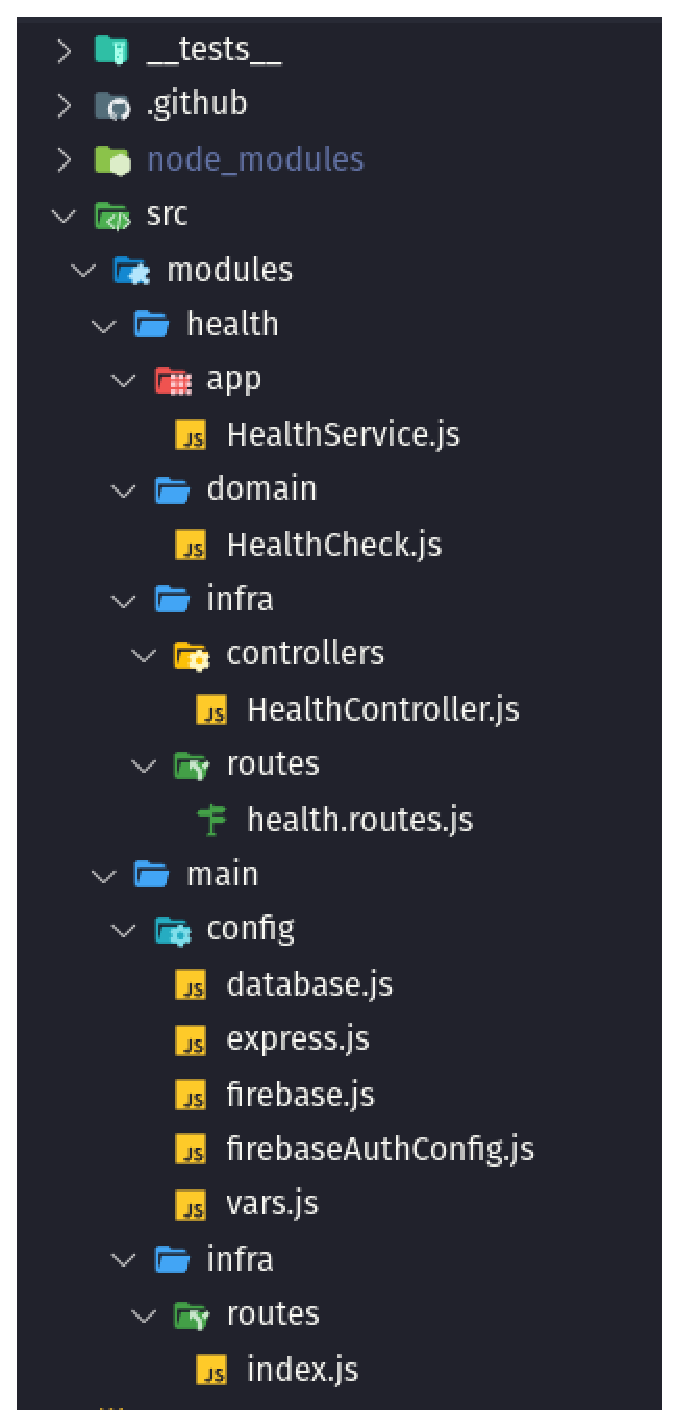
\includegraphics[keepaspectratio=true,scale=0.6]{figuras/poc1-pastas.eps}
	\parbox{\linewidth}{\centering FONTE: Autores}
	\label{fig-poc1-pastas}
\end{figure}

\subsubsection{Análise Quantitativa}

Este desafio incluiu a configuração da ferramenta SonarQube, que 
conforme abordado no capítulo de Suporte Tecnológico \ref{cap:suporte}, 
possibilita que a cada implementação de código para o projeto 
hospedado no GitHub, exista uma análise de qualidade do serviço. 
Diante disso, os insumos coletados por esta ferramenta após o desenvolvimento 
deste desafio podem ser vistos na tabela \ref{tab:poc1_sonarqube}.

\begin{table}[h]
  \centering
  \caption{Análise de qualidade do SonarQube sobre a POC 1}
  \begin{tabularx}{\linewidth}{l*{5}{>{\centering\arraybackslash}X}}
      \toprule
      \textbf{Métrica} & \textbf{Nota/Porcentagem} \\
      \midrule
      \rowcolor{gray!20} Confiabilidade & A \\
      Manutenibilidade & A \\
      \rowcolor{gray!20} Segurança & A \\
      Cobertura de Testes & 100\% \\
      \rowcolor{gray!20} Duplicações & 0\% \\
      \bottomrule
  \end{tabularx}
  \parbox{\linewidth}{\centering FONTE: Autores}
  \label{tab:poc1_sonarqube}
\end{table}

Observa-se que as métricas de Confiabilidade, Segurança e Manutenibilidade possuem nota A, 
indicando que não existem \textit{bugs} nem vulnerabilidades no sistema, e a 
quantidade de \textit{code smells} está menor que 5\%. Além disso, observa-se que a 
Cobertura de Testes se encontra em 100\% e a quantidade de 
Duplicações em 0\%, sendo excelentes notas para estes quesitos. Vale ressaltar que na 
configuração da Cobertura de Testes do SonarQube, foram incluídos na análise apenas os 
arquivos de implementação das funcionalidades, sendo não necessário testar os arquivos 
de configuração. Diante do exposto, conclui-se que esta solução está satisfatória para esta POC.


\section{POC 2 - Desenvolvimento do Cadastro e Login de Usuários}
\label{section:poc_2}

Essa seção aborda o desenvolvimento da \textit{feature}, relacionada ao cadastro de usuários dentro da 
plataforma do MiaAjuda. Inicialmente, é apresentada a Definição do Desafio \ref{section:poc_2_def_desafio} 
atrelada a essa prova de conceito, seguido pelos Requisitos do Desafio \ref{section:poc_2_req_desafio}.

\subsection{Definição do Desafio}
\label{section:poc_2_def_desafio}

Tem como objetivo desenvolver, utilizando o TDD, o cadastro e login de usuários na 
plataforma do MiaAjuda.

\subsubsection{Requisitos do Desafio}
\label{section:poc_2_req_desafio}

Para que a prova de conceito seja considerada finalizada, é necessário cumprir os seguintes requisitos:

\begin{itemize}
  \item O usuário deve ser capaz de efetuar seu cadastro;
  \item O usuário deve ser capaz de editar suas informações, e
  \item O usuário deve ser capaz de realizar login utilizando \textit{email} e senha cadastrados previamente.
\end{itemize}

\section{POC 3 - Desenvolvimento do Cadastro de Pedido de Ajuda}
\label{section:poc_3}

Essa seção aborda o desenvolvimento da \textit{feature} relacionada ao cadastro de pedidos de ajuda. 
Primeiramente, é apresentada a Definição do Desafio \ref{section:poc_3_def_desafio} atrelada a essa 
prova de conceito, seguido pelos Requisitos do Desafio \ref{section:poc_3_req_desafio}.

\subsection{Definição do Desafio}
\label{section:poc_3_def_desafio}

Tem como objetivo desenvolver, utilizando o TDD, o cadastro de pedidos de ajuda por 
parte de usuários que desejam ser ajudados.

\subsubsection{Requisitos do Desafio}
\label{section:poc_3_req_desafio}

Para que a prova de conceito seja considerada finalizada, é necessário cumprir os seguintes requisitos:

\begin{itemize}
  \item O usuário deve ser capaz de visualizar as categorias existentes;
  \item O usuário deve ser capaz de cadastrar um pedido de ajuda;
  \item O usuário deve ser capaz de visualizar seus respectivos pedidos de ajuda, e
  \item O usuário deve ser capaz de deletar um pedido de ajuda que pertence a ele.
\end{itemize}

\section{POC 4 - Desenvolvimento do Cadastro de Oferta de Ajuda}
\label{section:poc_4}

Essa seção aborda o desenvolvimento da \textit{feature} relacionada ao cadastro de ofertas de ajuda. 
Inicialmente, é apresentada a Definição do Desafio \ref{section:poc_4_def_desafio} atrelada a essa 
prova de conceito, seguido pelos Requisitos do Desafio \ref{section:poc_4_req_desafio}.

\subsection{Definição do Desafio}
\label{section:poc_4_def_desafio}

Tem como objetivo desenvolver, utilizando o TDD, o cadastro de oferta de ajuda por 
parte de usuários que desejam ajudar outros usuários.

\subsubsection{Requisitos do Desafio}
\label{section:poc_4_req_desafio}

Para que a prova de conceito seja considerada finalizada, é necessário cumprir os seguintes requisitos:

\begin{itemize}
  \item O usuário deve ser capaz de visualizar todos os pedidos de ajuda;
  \item O usuário deve ser capaz de filtrar os pedidos de ajuda por categoria, e
  \item O usuário deve ser capaz de oferecer ajuda para um pedido específico.
\end{itemize}

\section{Considerações Finais do Capítulo}
\label{section:consideracoes_finais_proposta}

Este capítulo teve o intuito de apresentar a proposta do trabalho, sendo: a reengenharia de um aplicativo utilizando 
as técnicas do TDD e DDD, descrevendo seu contexto, seguido da descrição do escopo da proposta e da documentação 
de cada prova de conceito necessária para alcançar o objetivo final do trabalho. Destaca-se que em cada prova de conceito, 
foram detalhados seus objetivos e seus respectivos requisitos. Além disso, foram apresentados os resultados 
iniciais obtidos com o desenvolvimento da POC 1 (\ref{section:poc_1}).
